\chapter{Visgoth System}\label{visgoth-ch}

The client-server architecture is a common model for interacting with remotely
stored datasets. There has been substantial work supporting the storage and
processing of large datasets \cite{hdfs} \cite{hadoop} \cite{spark}. However,
we find there is a gap when an analyst is attempting to access the stored data.
The size of storage and compute clusters allow petabyte scaling of datasets,
but a local client machine can only process a fraction of this data at any
given time. With the exception of mobile web designs, current architectures
ignore the heterogeneity among client hardware. When serving data to a client,
regardless of the current state of available client resources, the same dataset
is returned in response to a query. If a system were able to take the client
state into account, responses could be tailored to the individual client,
providing a more uniform response latency across clients. \\

Visgoth is a system aimed at dynamically changing a server response based on
profiling the state of the client and server machines. One use case is
visualization applications, in which the response data that the user views can
vary, since some degradation of data quality can be tolerated in return for low
latency responses. The way that a visualization is changed is an
application-specific trait, but could include downsampling or aggregating data
points. Visgoth provides profiling information about the current system state
to allow developers to adapt their results. \\

Examples where such a system would be valuable could be a data scientist
working with large amounts of time series data, for which coarser results are
acceptable for partial analysis. Another case could be a user viewing a social
media site with a low bandwidth connection. A text-only webpage or one with
limited multimedia could be an acceptable experience as opposed to no progress
being made while loading images. \\

We have built a prototype system to handle rendering the EEG spectrogram
visualizations in the browser.  We begin with related work in
Section~\ref{visgoth-ch:related-work}, followed by an outline of the design and
implementation in Sections~\ref{visgoth-ch:design} and
\ref{visgoth-ch:implementation}, experimental results in
Section~\ref{visgoth-ch:results}, future work in
Section~\ref{discuss-ch:visgoth-future-work}.

\section{Related Work}\label{visgoth-ch:related-work}

Currently, no visualization library takes advantage of information about the
client's real-time state, only the more static hardware configuration. There
has, however, been substantial research on optimizing performance of large
dataset visualization. \\

Interactive querying of multidimensional dataset visualization was explored by
the \emph{imMens} project \cite{immens}, a web-based visualization library with
a server-client architecture. \emph{imMens} was able to achieve higher
performance for data interaction through preprocessing of large
multidimensional data cubes. Data was decomposed into data tiles, or subsets of
the larger dataset, which turned out to be more flexible to compute on and
serve to the client. \\

Similarly, the \emph{M4} system \cite{m4} uses an aggregation-based time series
dimensionality reduction technique to provide error-free visualizations at high
data reduction rates. This system targets particular data reduction techniques,
but does not account for client heterogeneity or varying system resources to
apply the reductions. \\

The \emph{ForeCache} system \cite{forecache} uses predictive models based on
recent user interactions and requested data characteristics (e.g. histograms)
to prefetch similar data tiles for display. This system is able to adaptively
serve visualizations to the client, but currently only accounts for user
behavior, not differences in the clients' machines. Also, while
\emph{ForeCache} can choose which tiles to prefetch, it does not ever adjust
the tile size itself.\\

\emph{BigDawg} \cite{bigdawg} is a big data storage system with proposed solutions
for visualization interfaces. It is currently under development and affirms the
need for a large-scale visualization system. Part of the motivation for
BigDawg's visualization interface is the need for an analyst to `drill down'
into datasets, interactively choosing portions to focus on and smoothly panning
and zooming among these sections. \\

The work done by Lee, Ko, and Fox \cite{adapting-heterogeneous} addresses
adapting content for mobile devices.  This is done through a series of
``transcoding'' techniques, essentially data reductions on different types of
media content based on the client hardware.  The system bases transcoding
operations on client hardware types, but does not take into account client
resource state that change over time, such as network connectivity or
bandwidth.\\

\section{Design}\label{visgoth-ch:design}

The Visgoth system is split into three main components: the Visgoth server, the
application server, and the application client (the web browser). The lifetime
of a client interaction in an application using Visgoth can be split into two
phases: request and response. \\

First, during the request phase, profiling information about current
performance is collected on both the client and the application server. These
statistics are sent to the Visgoth server, which uses static regression models
to predict a data reduction factor. The application server then uses the data
reduction factor to adapt the visualizations that the client receives. In
Figure~\ref{fig:system-request}, we show an example request that the Visgoth
server would receive. The request inludes the normal application request
parameters that are used to request a visualiation, along with the Visgoth
profiling information (highlighted).\\

\begin{figure}[h]
\begin{center}
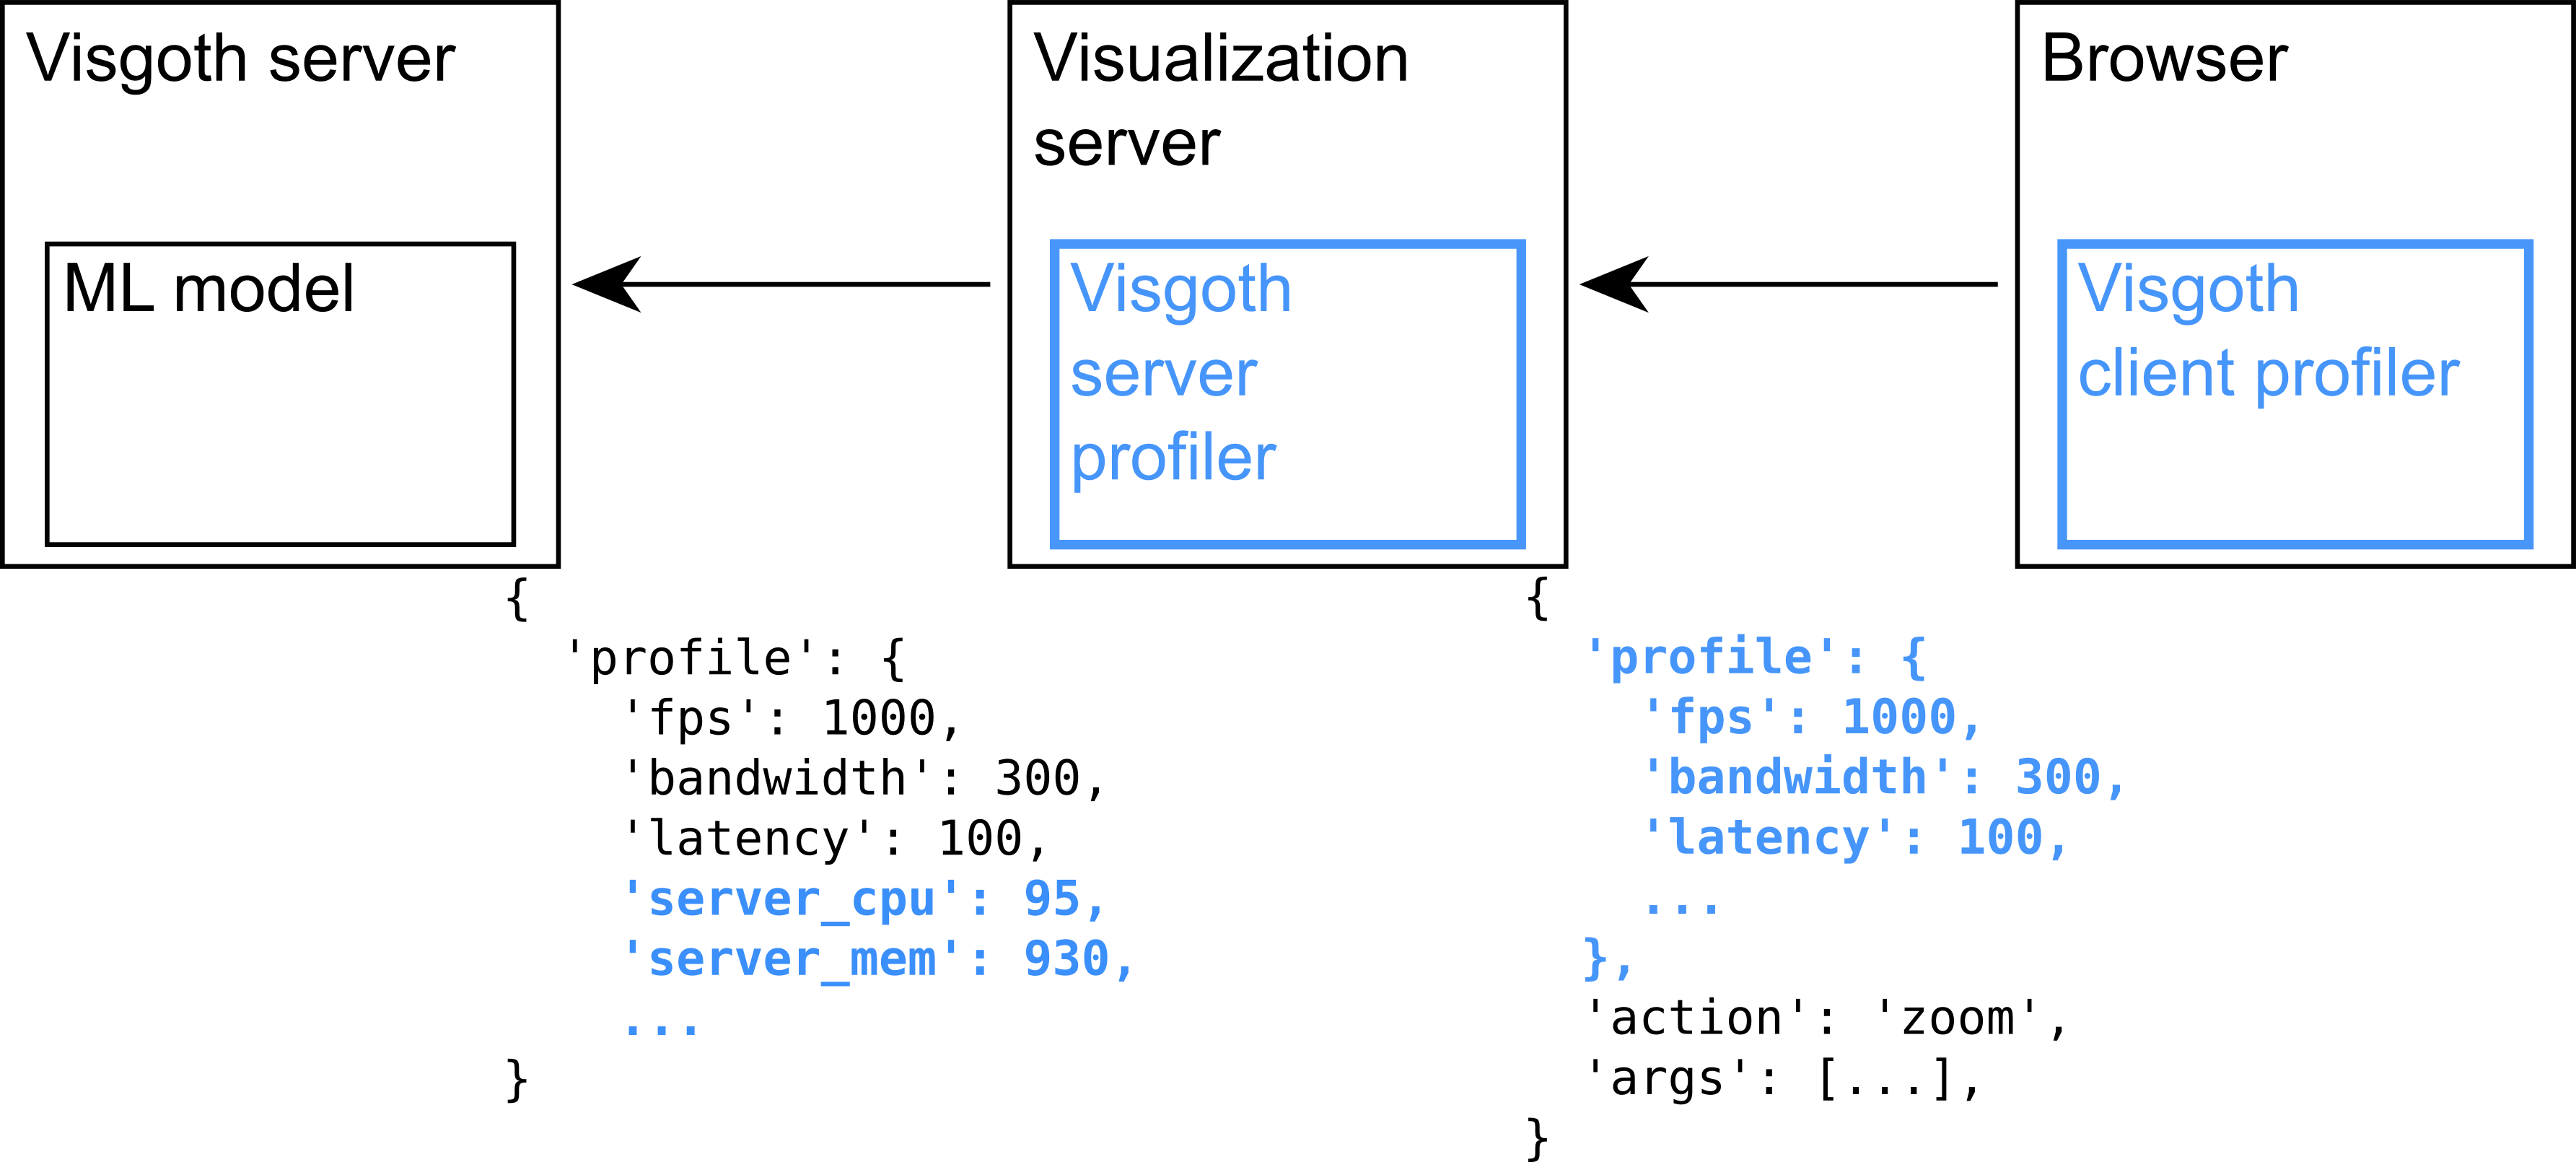
\includegraphics[scale=0.5]{./img/system-request.png}
\caption{Sample request in the Visgoth system.}
\label{fig:system-request}
\end{center}
\end{figure}

Second, during the response phase, the Visgoth server uses the regression model
to suggest a data reduction factor to the application server.
Figure~\ref{fig:system-response} shows an example response from the Visgoth
server, which suggests a data reduction by a factor (extent) of 10. The
application server then applies this reduction, serving coarser data to the
client. In the context of the visualization application, this would be
equivalent to the application server sending a blurrier image back to the
browser.\\

\begin{figure}[h]
\begin{center}
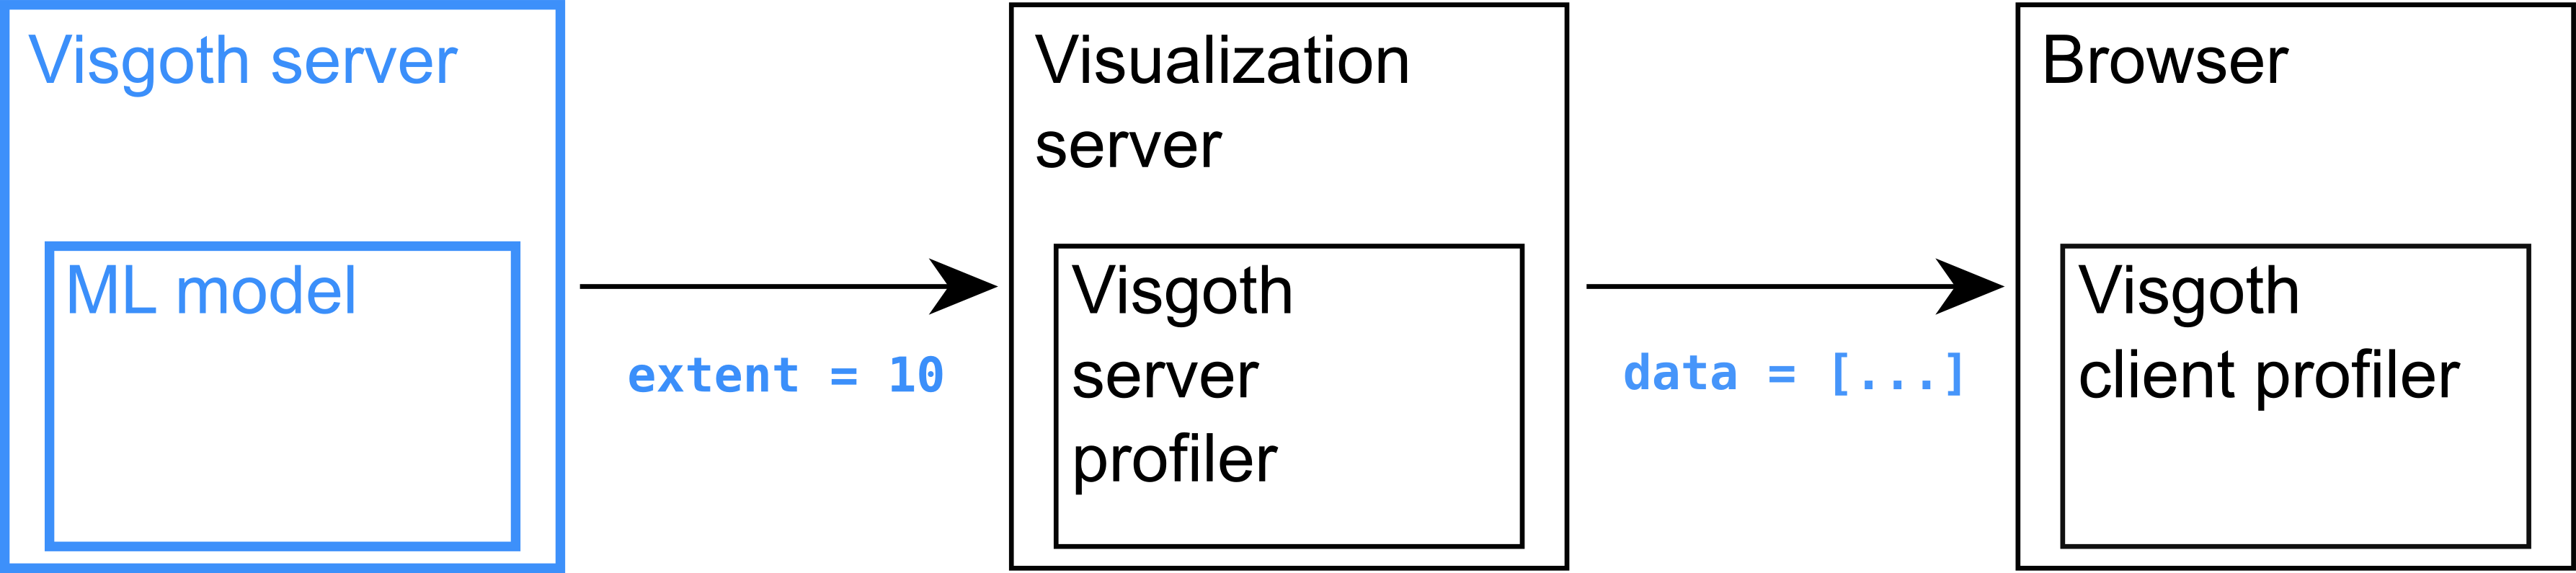
\includegraphics[scale=0.5]{./img/system-response.png}
\caption{Sample response in the Visgoth system.}
\label{fig:system-response}
\end{center}
\end{figure}

In the following sections, we describe these two phases in more detail. In
Section~\ref{visgoth-ch:profile-collection}, we discuss the Visgoth profilers that are
installed in the application server and client. In Section~\ref{visgoth-ch:modeling}, we
discuss how the Visgoth server uses this information to predict a data
reduction factor.\\

  \subsection{Profile Collection}\label{visgoth-ch:profile-collection}

  Profile collection is needed for both the initial training of the Visgoth
  regression model, as well as the actual application requests. These two
  phases of profile collection are essentially the same, except that during the
  training phase, the Visgoth server sets a default data reduction factor,
  versus a predicted factor during the application phase. Eventually, Visgoth's
  regression model could be made dynamic by also training on incoming
  application requests, but dividing profile collection into two phases is
  simpler to implement for this prototype.\\

  Profiling information is collected both at the client and the server to
  capture different types of data. We collect profiling information from three
  different categories: static, dynamic and application specific data.  Static
  data such as the client or server hardware is useful, especially since the
  client hardware can be heterogeneous. This allows Visgoth to fine tune it's
  models based on the hardware being used. Dynamic system statistics such as
  network or memory usage allow Visgoth to make up-to-date prediction
  decisions. Finally, application specific profiling such as rendering or
  computation time allow a developer to choose which factors are most important
  on an application basis.\\

  On both the client and server, Visgoth allows the developer to set a default
  \emph{window} size for individual statistics. This indicates to the Visgoth
  profilers how many of the most recent samples for a profile statistic to keep
  track of. The idea behind using a time-based \emph{window} is to keep a
  running average of the most recent profile values, but not to keep it so
  large that the values sent to the Visgoth server are no longer relevant.\\

  In general, profile information on the application server is easier to
  collect because the developer should have direct access to the server's
  machine. There is already widespread support for profiling a local machine,
  which we discuss in more detail in Section~\ref{visgoth-ch:implementation-server}. Here,
  we focus instead on the more difficult case of collecting information on the
  client.\\

  \subsubsection{Client Profiler}

  Profiling the client is tricky because, for security reasons, most browsers
  purposefully do not expose information about the client machine. Certain
  pieces of static information are readily available, such as the browser and
  machine type from the ``User-Agent'' string, assuming that the client does
  not mock it.  However, static hardware information such as the RAM size is in
  general inaccessible, to our best knowledge.\\

  The Visgoth client profiler has better support for application-specific
  dynamic profiling.  Most modern browsers support \c{window.performance}, a
  high-resolution time data API that allows a web client to set marks and get
  the current timestamp (see Section~\ref{visgoth-ch:implementation-client}). With this
  API, we are able to get real-time information about the network and where in
  the code the client spends most of its time.\\

  We can get approximate numbers for network latency and network bandwidth by
  using the \c{window.performance} API and slightly modifying the application
  server. Because the client and server's clocks are not synced, the best that
  we can do is measure the total round-trip time between the client's request
  and the client's receipt of the response. In that case, we do not want to
  measure an actual application request's time since this would likely include
  extra computation on the server side that the client cannot measure. Instead,
  we can make a small modification to the application server to include a dummy
  endpoint that serves a small static piece of nonsense data. The portion of
  time on server computation for such a request is unlikely to be significant
  relative to the overall request time.\\

  Assuming some margin of error, we can now profile the network by sending
  dummy requests to the application server. The network latency is equal to
  the round-trip time. The network bandwidth is equal to the size of the
  request and response packets divided by the round-trip time.\\

  Network health can vary significantly across time. In order to get accurate
  real-time statistics, the client must poll the application server with the
  dummy requests more frequently than it would send normal application
  requests, which are triggered by user interactions. However, the client
  should not poll the network so often that it interferes with the
  application's overall latency. Similarly, the nonsense data that the server
  returns should not be so large that it dominates the client's bandwidth. A
  developer using Visgoth will have to tune the polling rate and the size of
  the response data to make sure there is no noticeable difference in their
  application. Eventually, Visgoth could also vary the size of the response
  data, using the same data reduction factor that it predicts according to
  current profile information.\\

  In addition to the network, Visgoth can collect profiling information about
  client-side computation, again using the \c{window.performance} API.
  Visgoth exposes a higher-level \c{statistic} API to the developer.  The
  developer can produce instances of \c{statistic}, each of which has a
  tag and \c{begin()} and \c{end()} methods that the developer can
  use to mark the beginning and end of the procedure that they want to profile.
  When \c{statistic.end()} is called, the \c{statistic} dumps the
  measured time since \c{statistic.begin()} was called for the same
  instance to Visgoth's global state.\\

  This simple API is sufficient to measure throughput information as well as
  latency. For instance, in a visualization application, one can measure the
  frames rendered per second. This is done by counting the number of frames
  rendered within some time interval and dividing by the rendering time,
  which can be measured using the Visgoth \c{statistic} API.\\

  \subsection{Modeling}\label{visgoth-ch:modeling}

  Visgoth's goal overall is to provide a uniform experience across all clients,
  no matter the hardware or workload variation across the clients. To do this,
  Visgoth must be able to predict what the total \emph{latency} of a particular
  application request will be. Here, \emph{latency} does not refer to the
  network, but to the time between the client interaction, e.g. a click on a
  webpage, and the time when the results are visible in the browser, e.g. an
  image is rendered. We hope that providing a uniform \emph{latency}, while
  still serving as high of a data resolution as possible, will translate to a
  more uniform experience across all clients.\\

  Visgoth predicts \emph{latency} using a set of pre-trained regression models,
  one for each value of \emph{downsample}, the factor that the application
  server reduces its data by. The features of each model comprise of the
  statistics from the profiles collected on the application server and client.
  We train a single regression model by setting a default value for
  \emph{downsample} and running an application request for a set number of
  trials to get variation in the profiles.\\

  Once the regression models are trained, the learning goal can be framed as
  follows: Given a current profile of the application server and client and a
  target value for \emph{latency}, predict the value of \emph{downsample} that
  will reach the closest to target \emph{latency} value. More formally, Visgoth
  starts with a set of regression models $\{ M_1, \dots, M_n \}$, where each
  $M_i$ is of the form:

  \begin{equation*}
    M_i(P) = latency
  \end{equation*}

  Here, $i$ is the value of \emph{downsample} during the application requests
  that model $M_i$ was trained on. $P$ is a feature vector, containing all the
  statistics from the application server and client profiles. \emph{latency} is
  the predicted latency if the current profile is $P$ and the application
  server reduces data served by a factor of $i$.\\

  Visgoth takes as input a profile $P$ from the application server and client.
  Visgoth does not simply minimize \emph{latency}, or else it would always send
  the least data possible. Instead, our goal is to strike a balance between
  \emph{latency} and the quality of the client's results. To do this, we
  instead try to minimize the difference between the actual latency experienced
  and a target value $l$ for \emph{latency}. To determine what value of
  \emph{downsample} the application server should use, Visgoth computes the $i$
  that minimizes the distance between the predicted latency and $l$:

  \begin{equation*}
    \mid M_i(P) - l \mid
  \end{equation*}

\section{Implementation}\label{visgoth-ch:implementation}

  \subsubsection{Server Profiler}\label{visgoth-ch:implementation-server}

  The server profile collects statistics concerning the server state or
  calculations. For the EEG application we use statistics recorded by the
  \c{collectd} \cite{collectd} library. We keep statistics pertaining to free
  memory, user CPU, network and disk usage to monitor server load.  Load could
  be increased by additional clients connecting or server resources being
  consumed by other server programs.

  \subsubsection{Client Profiler}\label{visgoth-ch:implementation-client}

  The \c{window.performance} high-resolution time data API proved to be
  essential for gaining client profile information. \c{window.performance} is a
  widely supported API that provides functions for timing webpages. We used two
  main methods, \c{mark()} and \c{now()} to build the higher-level Visgoth
  \c{statistic} API. The \c{mark()} method can be used to set and name a mark
  at the time that it is called. The \c{now()} method returns the current
  timestamp, which can be used to measure against marks. These together can be
  used to measure different spans of application client code.

\section{Results}\label{visgoth-ch:results}

We ran experiments using the CSAIL OpenStack infrastructure to host the
visualization server and using our local machines as clients. The server,
running Ubuntu 14.04.3, had 4 cores available with 8GB of RAM and Intel Xeon
2.27GHz processors. The client machine ran Ubuntu 14.04.3, and experiments were
run in both Google Chrome (46.0.2490.86) and Mozilla Firefox (42.0). \\

We predicted that \emph{latency} would correlate with \emph{downsample}, since
in general, if less data is sent, it is likely to take less time on the
network. However, we also predicted that \emph{downsample} wasn't the only
factor in \emph{latency}. This would indicate that there are application
server- and client-specific factors also at play.

  \begin{figure}[h]
  \begin{center}
  \begin{subfigure}{0.49\textwidth}
    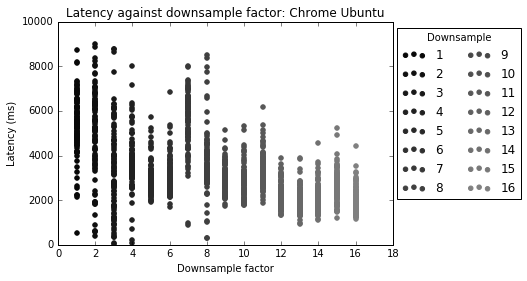
\includegraphics[width=\textwidth]{./img/chrome-extent.png}
    \caption{Chrome}
  \end{subfigure}
  \begin{subfigure}{0.49\textwidth}
    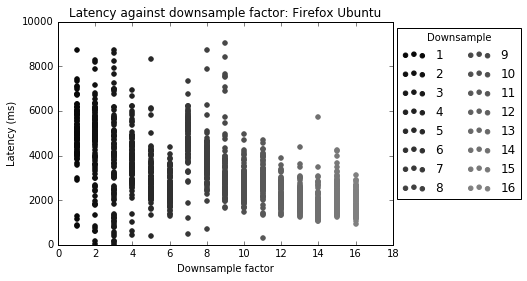
\includegraphics[width=\textwidth]{./img/firefox-extent.png}
    \caption{Firefox}
  \end{subfigure}
  \caption{Overall \emph{latency} of an application client's interaction,
      plotted against \emph{downsample}, the factor by which the application
      server reduced data served back to the client.}
  \label{fig:extent}
  \end{center}
  \end{figure}

To validate this prediction, we ran the same request on the visualization
application 100 times each for \emph{downsample} values from 1 to 16. We
recorded the profile and total \emph{latency} for each request. In
Figure~\ref{fig:extent}, there is indeed a downward trend in \emph{latency} as
\emph{downsample} increases. However, there is also significant variation in
\emph{latency} across all columns. In fact, every value tested for
\emph{downsample} achieved a \emph{latency} of about 3 seconds for at least one
application request. We can conclude from this data that there are indeed other
factors that determine the variation in \emph{latency} besides just
\emph{downsample}.\\

Although we'd hoped to build a model on all of the features in the server and
client profile, we chose for the sake of time to focus on a single feature in
order to quickly validate the Visgoth system's utility. We looked for a single
feature that shared a strong correlation with \emph{latency}.\\

  \begin{figure}[h]
  \begin{center}
  \begin{subfigure}{0.49\textwidth}
    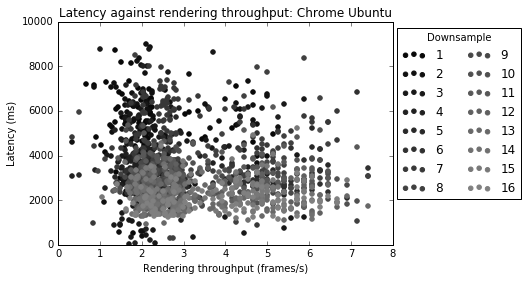
\includegraphics[width=\textwidth]{./img/chrome-fps.png}
    \caption{Chrome}
  \end{subfigure}
  \begin{subfigure}{0.49\textwidth}
    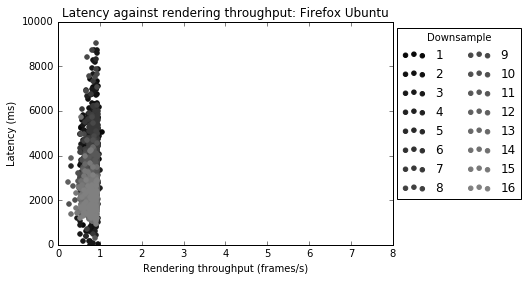
\includegraphics[width=\textwidth]{./img/firefox-fps.png}
    \caption{Firefox}
  \end{subfigure}
  \caption{Overall \emph{latency} of an application client's interaction,
      plotted against rendering throughput, the number of spectrogram frames
      that can be rendered per second.}
  \label{fig:fps}
  \end{center}
  \end{figure}

We first looked at rendering throughput, measured by taking the inverse of the
time needed to render a single frame of the spectrogram. The results are shown
in Figure~\ref{fig:fps}. We can conclude that Firefox in general has a much
more consistent and lower rendering throughput than Chrome.  However, as was
the case for \emph{downsample}, rendering throughput does not seem to correlate
with \emph{latency}. This shows us that for this particular application,
rendering time is unlikely to be a bottleneck.\\


Finally, we did the same with \emph{latency} versus bandwidth, shown in
Figure~\ref{fig:bandwidth}. Just by visual inspection, bandwidth clearly had
the strongest correlation with \emph{latency}, so we decided to train
regression models on this profile feature. We used a robust Theil-Sen
regression, fit to an equation of the form:

\begin{equation*}
  latency = a + \frac{b}{bandwidth}
\end{equation*}

We used 75\% of our dataset of 1600 points to train the 16 regression models,
one for each $downsample$ value. The coefficient of determination $R^2$ was
0.71 for model $M_1$, for which there was no data reduction, and over 0.99 for
the other 15 models. Figure~\ref{fig:bandwidth} shows a selection of these
models, including $M_1$, along with the test dataset points.\\

  \begin{figure}[h]
  \begin{center}
  \begin{subfigure}{0.49\textwidth}
    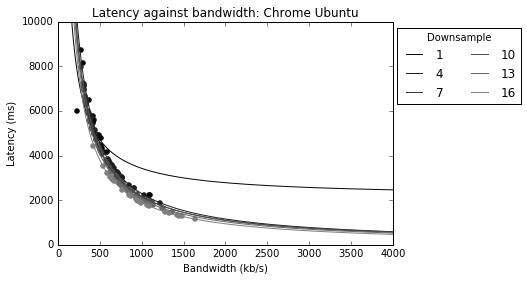
\includegraphics[width=\textwidth]{./img/chrome-bandwidth.png}
    \caption{Chrome}
  \end{subfigure}
  \begin{subfigure}{0.49\textwidth}
    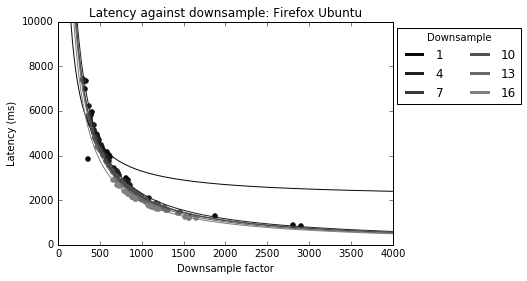
\includegraphics[width=\textwidth]{./img/firefox-bandwidth.png}
    \caption{Firefox}
  \end{subfigure}
  \caption{Overall \emph{latency} of an application client's interaction,
      plotted against approximate network bandwidth. Each curve represents the
      \emph{latency} values predicted by one regression model. The points
      plotted are from the test dataset.}
    \label{fig:bandwidth}
  \end{center}
  \end{figure}

The curve for $M_1$ predicts a much higher \emph{latency} for higher bandwidths
than the other models, while the other models also predict similar
\emph{latency} values. This indicates that at these bandwidths, Visgoth will
almost always recommend some data reduction. This may not be so useful to an
application developer, who could just set a default \emph{downsample} factor
without Visgoth. \\

However, at lower bandwidths, around 500 KB/s, the same bandwidth is predicted
to produce different latencies depending on which \emph{downsample} value is
used. This is where the Visgoth system could have impact on the client's
experience. Within this range of bandwidths, it is unclear from a developer's
perspective which default value of \emph{downsample} would always produce the
target \emph{latency} value, or if there even is one.\\

To validate Visgoth's utility at these lower bandwidths, we reran the same
experiment, but this time using the \emph{downsample} value predicted by the
Visgoth server. We set a target \emph{latency} of 4 seconds. For this
experiment, we hoped to see \emph{latency} values that were uniform relative to
those in Figure~\ref{fig:extent}. The latencies also should have been centered
at our target value across all application requests, regardless of the
\emph{downsample} factor set by Visgoth.\\

Unfortunately, we did not see an appreciable difference in \emph{latency}
variation from Figure~\ref{fig:extent}. However, we believe that this is due to
our experiment setup. We were unable to implement frequent polling of the
network in time for this experiment. Instead, we used the bandwidth measured
during the previous request as the ``current'' bandwidth profile. We waited 9
seconds between requests to give the application time to receive a response,
meaning that the bandwidth profile used to predict the \emph{downsample} for
each request was actually from 9 seconds ago. In order to get more meaningful
results, it will be necessary to send Visgoth more recent profiling
information.

